\section{Ressursplanlegging (Oppgave 1)}
	
	{\bf Oppgave 1A) Construer prosjektets AON nettverk} \\
	I figuren nedenfor vises AON nettverket med alle tidligste og seneste start/slutt tid.

	{\bf Oppgave 1B) Identifiser kritisk sti og alle andre mulige stier gjennom nettverket.} \\

	\begin{itemize}
		\item A - B - E - H 
		\item {\color{red} A - C - D - F - H (critical path)}
		\item A - B - D - F - H 
		\item A - C - G - H 
	\end{itemize}

	{\bf Opphave 1C) Lag ressursfordelingsplan med tidlig og sen start} \\

		Se figure 2  for tabell. Den er delt inn i uker og tallene i rutene er
		antall ressurstimer som blir brukt hver uke. Tallene i bold viser 
		tidligste start-slutt, mens tallene i parentes viser seneste start-slutt for
		hver aktivitet.
		De 3 nederste radene viser antall ressurstimer pr uke. 
		Første raden viser med utgangspunkt med tidligste start (ES) og rad 2 viser
		med utgangspunkt i seneste start (LS).

	{\bf Oppgave 1D) Anta at max arbeid pr uke er 8 ressurstimer. Er det noen uker som overskrider dette?} \\

		Hvis vi tar utgangspunkt i tidlig start ser vi at uke 10 og 11 ligger på 11 ressurstimer!


	{\bf Oppgave 1E) Omgjør på fordelingen slik at ingen uker overskrider 8 ressurstimer.} \\

		I figure 2, nederste rad viser forslag på hvordan timene kan fordeles. Det vi har gjort
		er å ta utgangspunkt i tidlig start (ES), bortsett fra aktivitet G som bruker late start.


	\begin{figure}[H]
		\centering
		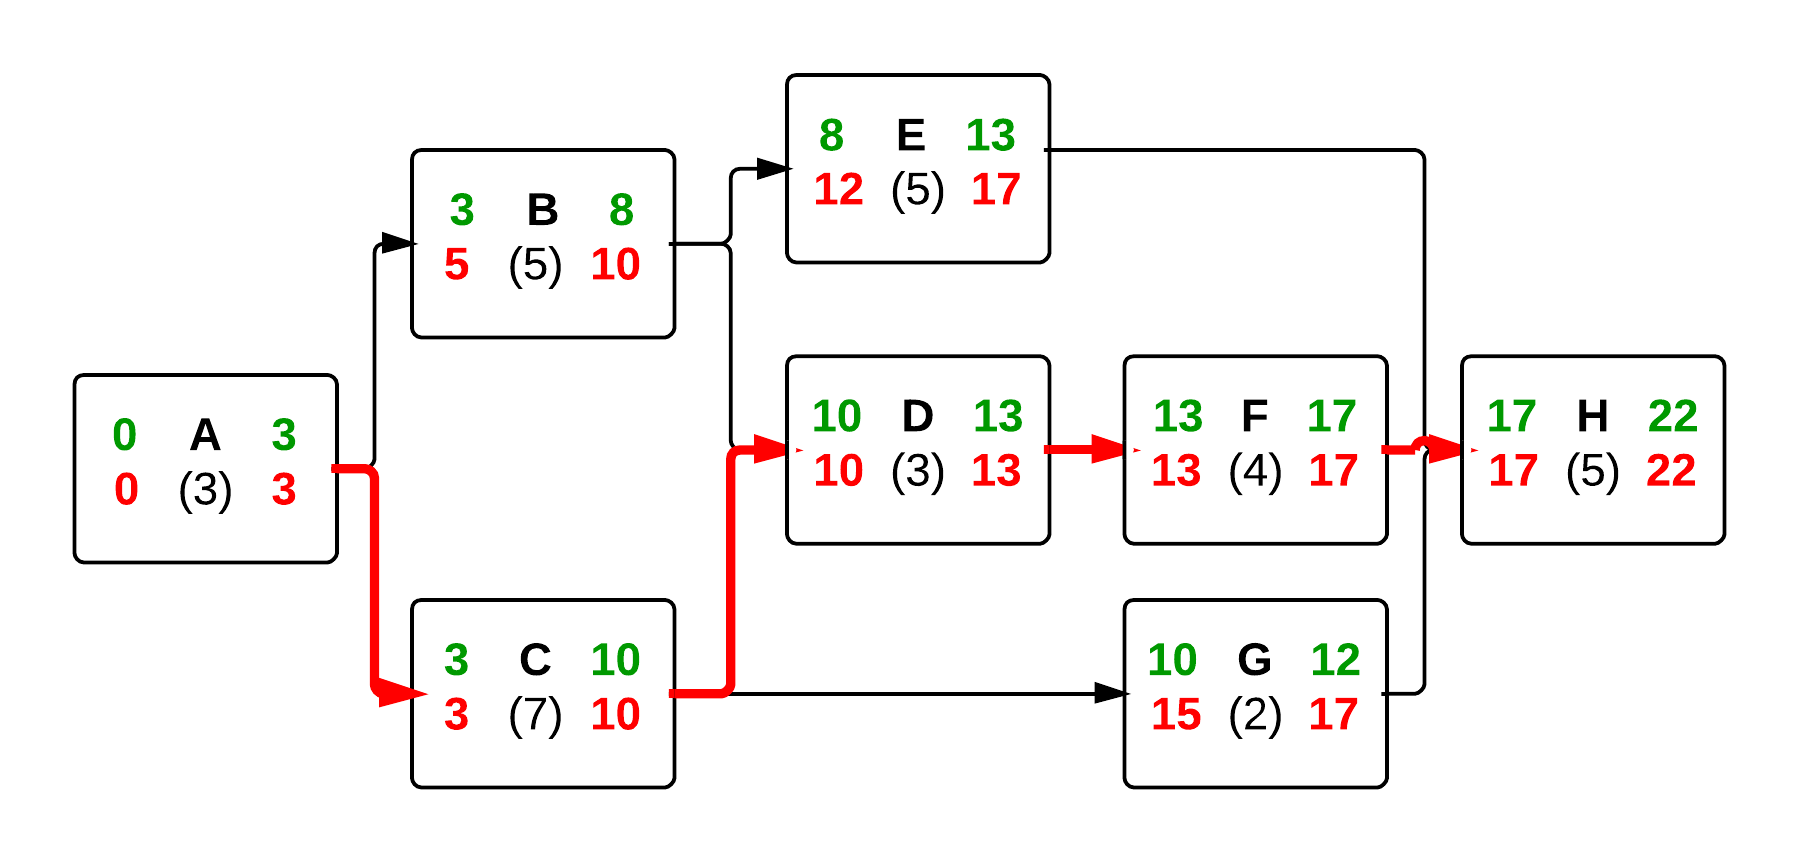
\includegraphics[scale=0.3, angle=90]{task2.png}
		\caption{AON nettverk}
	\end{figure}

	\begin{figure}[H]
		\centering
		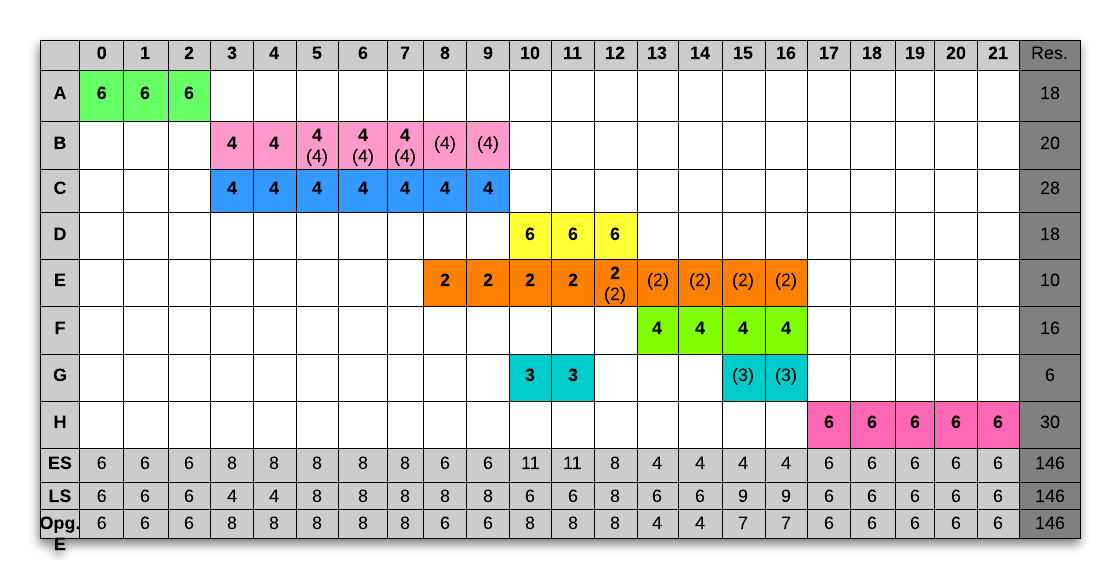
\includegraphics[scale=0.55, angle=90]{task1.png}
		\caption{Ressurstabell}
	\end{figure}